% Generated by ArticleSignalDiagrams. Opaque vector fills only.
\documentclass[10pt,tikz,border=5pt]{standalone}
\usepackage{lmodern}
\usetikzlibrary{fit}
\begin{document}
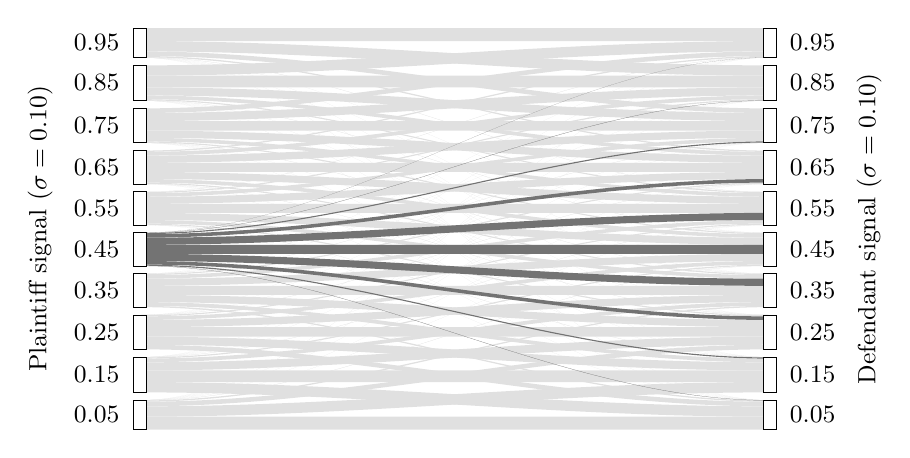
\begin{tikzpicture}[x=1cm,y=1cm,font=\small]\path[fill=black!12,draw=none] (3.3,-5.1) .. controls (6,-5.1) and (8.6,-5.1) .. (11.3,-5.1) -- (11.3,-4.93582) .. controls (8.6,-4.93582) and (6,-4.93582) .. (3.3,-4.93582) -- cycle;
\path[fill=black!12,draw=none] (3.3,-4.93582) .. controls (6,-4.93582) and (8.6,-4.626347) .. (11.3,-4.626347) -- (11.3,-4.494901) .. controls (8.6,-4.494901) and (6,-4.804374) .. (3.3,-4.804374) -- cycle;
\path[fill=black!12,draw=none] (3.3,-4.804374) .. controls (6,-4.804374) and (8.6,-4.079804) .. (11.3,-4.079804) -- (11.3,-4.021371) .. controls (8.6,-4.021371) and (6,-4.745941) .. (3.3,-4.745941) -- cycle;
\path[fill=black!12,draw=none] (3.3,-4.745941) .. controls (6,-4.745941) and (8.6,-3.543851) .. (11.3,-3.543851) -- (11.3,-3.527622) .. controls (8.6,-3.527622) and (6,-4.729712) .. (3.3,-4.729712) -- cycle;
\path[fill=black!12,draw=none] (3.3,-4.729712) .. controls (6,-4.729712) and (8.6,-3.020431) .. (11.3,-3.020431) -- (11.3,-3.017453) .. controls (8.6,-3.017453) and (6,-4.726734) .. (3.3,-4.726734) -- cycle;
\path[fill=black!12,draw=none] (3.3,-4.726734) .. controls (6,-4.726734) and (8.6,-2.5) .. (11.3,-2.5) -- (11.3,-2.499642) .. controls (8.6,-2.499642) and (6,-4.726376) .. (3.3,-4.726376) -- cycle;
\path[fill=black!12,draw=none] (3.3,-4.726376) .. controls (6,-4.726376) and (8.6,-1.979569) .. (11.3,-1.979569) -- (11.3,-1.979541) .. controls (8.6,-1.979541) and (6,-4.726348) .. (3.3,-4.726348) -- cycle;
\path[fill=black!12,draw=none] (3.3,-4.726348) .. controls (6,-4.726348) and (8.6,-1.456149) .. (11.3,-1.456149) -- (11.3,-1.456148) .. controls (8.6,-1.456148) and (6,-4.726347) .. (3.3,-4.726347) -- cycle;
\path[fill=black!12,draw=none] (3.3,-4.726347) .. controls (6,-4.726347) and (8.6,-0.920196) .. (11.3,-0.920196) -- (11.3,-0.920196) .. controls (8.6,-0.920196) and (6,-4.726347) .. (3.3,-4.726347) -- cycle;
\path[fill=black!12,draw=none] (3.3,-4.726347) .. controls (6,-4.726347) and (8.6,-0.373653) .. (11.3,-0.373653) -- (11.3,-0.373653) .. controls (8.6,-0.373653) and (6,-4.726347) .. (3.3,-4.726347) -- cycle;
\path[fill=black!12,draw=none] (3.3,-4.626347) .. controls (6,-4.626347) and (8.6,-4.93582) .. (11.3,-4.93582) -- (11.3,-4.804374) .. controls (8.6,-4.804374) and (6,-4.494901) .. (3.3,-4.494901) -- cycle;
\path[fill=black!12,draw=none] (3.3,-4.494901) .. controls (6,-4.494901) and (8.6,-4.494901) .. (11.3,-4.494901) -- (11.3,-4.347983) .. controls (8.6,-4.347983) and (6,-4.347983) .. (3.3,-4.347983) -- cycle;
\path[fill=black!12,draw=none] (3.3,-4.347983) .. controls (6,-4.347983) and (8.6,-4.021371) .. (11.3,-4.021371) -- (11.3,-3.918577) .. controls (8.6,-3.918577) and (6,-4.24519) .. (3.3,-4.24519) -- cycle;
\path[fill=black!12,draw=none] (3.3,-4.24519) .. controls (6,-4.24519) and (8.6,-3.527622) .. (11.3,-3.527622) -- (11.3,-3.479983) .. controls (8.6,-3.479983) and (6,-4.197551) .. (3.3,-4.197551) -- cycle;
\path[fill=black!12,draw=none] (3.3,-4.197551) .. controls (6,-4.197551) and (8.6,-3.017453) .. (11.3,-3.017453) -- (11.3,-3.002932) .. controls (8.6,-3.002932) and (6,-4.183029) .. (3.3,-4.183029) -- cycle;
\path[fill=black!12,draw=none] (3.3,-4.183029) .. controls (6,-4.183029) and (8.6,-2.499642) .. (11.3,-2.499642) -- (11.3,-2.496798) .. controls (8.6,-2.496798) and (6,-4.180185) .. (3.3,-4.180185) -- cycle;
\path[fill=black!12,draw=none] (3.3,-4.180185) .. controls (6,-4.180185) and (8.6,-1.979541) .. (11.3,-1.979541) -- (11.3,-1.979189) .. controls (8.6,-1.979189) and (6,-4.179833) .. (3.3,-4.179833) -- cycle;
\path[fill=black!12,draw=none] (3.3,-4.179833) .. controls (6,-4.179833) and (8.6,-1.456148) .. (11.3,-1.456148) -- (11.3,-1.45612) .. controls (8.6,-1.45612) and (6,-4.179805) .. (3.3,-4.179805) -- cycle;
\path[fill=black!12,draw=none] (3.3,-4.179805) .. controls (6,-4.179805) and (8.6,-0.920196) .. (11.3,-0.920196) -- (11.3,-0.920195) .. controls (8.6,-0.920195) and (6,-4.179804) .. (3.3,-4.179804) -- cycle;
\path[fill=black!12,draw=none] (3.3,-4.179804) .. controls (6,-4.179804) and (8.6,-0.373653) .. (11.3,-0.373653) -- (11.3,-0.373653) .. controls (8.6,-0.373653) and (6,-4.179804) .. (3.3,-4.179804) -- cycle;
\path[fill=black!12,draw=none] (3.3,-4.079804) .. controls (6,-4.079804) and (8.6,-4.804374) .. (11.3,-4.804374) -- (11.3,-4.745941) .. controls (8.6,-4.745941) and (6,-4.021371) .. (3.3,-4.021371) -- cycle;
\path[fill=black!12,draw=none] (3.3,-4.021371) .. controls (6,-4.021371) and (8.6,-4.347983) .. (11.3,-4.347983) -- (11.3,-4.24519) .. controls (8.6,-4.24519) and (6,-3.918577) .. (3.3,-3.918577) -- cycle;
\path[fill=black!12,draw=none] (3.3,-3.918577) .. controls (6,-3.918577) and (8.6,-3.918577) .. (11.3,-3.918577) -- (11.3,-3.79879) .. controls (8.6,-3.79879) and (6,-3.79879) .. (3.3,-3.79879) -- cycle;
\path[fill=black!12,draw=none] (3.3,-3.79879) .. controls (6,-3.79879) and (8.6,-3.479983) .. (11.3,-3.479983) -- (11.3,-3.388036) .. controls (8.6,-3.388036) and (6,-3.706843) .. (3.3,-3.706843) -- cycle;
\path[fill=black!12,draw=none] (3.3,-3.706843) .. controls (6,-3.706843) and (8.6,-3.002932) .. (11.3,-3.002932) -- (11.3,-2.957445) .. controls (8.6,-2.957445) and (6,-3.661355) .. (3.3,-3.661355) -- cycle;
\path[fill=black!12,draw=none] (3.3,-3.661355) .. controls (6,-3.661355) and (8.6,-2.496798) .. (11.3,-2.496798) -- (11.3,-2.482505) .. controls (8.6,-2.482505) and (6,-3.647063) .. (3.3,-3.647063) -- cycle;
\path[fill=black!12,draw=none] (3.3,-3.647063) .. controls (6,-3.647063) and (8.6,-1.979189) .. (11.3,-1.979189) -- (11.3,-1.976358) .. controls (8.6,-1.976358) and (6,-3.644231) .. (3.3,-3.644231) -- cycle;
\path[fill=black!12,draw=none] (3.3,-3.644231) .. controls (6,-3.644231) and (8.6,-1.45612) .. (11.3,-1.45612) -- (11.3,-1.455769) .. controls (8.6,-1.455769) and (6,-3.64388) .. (3.3,-3.64388) -- cycle;
\path[fill=black!12,draw=none] (3.3,-3.64388) .. controls (6,-3.64388) and (8.6,-0.920195) .. (11.3,-0.920195) -- (11.3,-0.920167) .. controls (8.6,-0.920167) and (6,-3.643852) .. (3.3,-3.643852) -- cycle;
\path[fill=black!12,draw=none] (3.3,-3.643852) .. controls (6,-3.643852) and (8.6,-0.373653) .. (11.3,-0.373653) -- (11.3,-0.373652) .. controls (8.6,-0.373652) and (6,-3.643851) .. (3.3,-3.643851) -- cycle;
\path[fill=black!12,draw=none] (3.3,-3.543851) .. controls (6,-3.543851) and (8.6,-4.745941) .. (11.3,-4.745941) -- (11.3,-4.729712) .. controls (8.6,-4.729712) and (6,-3.527622) .. (3.3,-3.527622) -- cycle;
\path[fill=black!12,draw=none] (3.3,-3.527622) .. controls (6,-3.527622) and (8.6,-4.24519) .. (11.3,-4.24519) -- (11.3,-4.197551) .. controls (8.6,-4.197551) and (6,-3.479983) .. (3.3,-3.479983) -- cycle;
\path[fill=black!12,draw=none] (3.3,-3.479983) .. controls (6,-3.479983) and (8.6,-3.79879) .. (11.3,-3.79879) -- (11.3,-3.706843) .. controls (8.6,-3.706843) and (6,-3.388036) .. (3.3,-3.388036) -- cycle;
\path[fill=black!12,draw=none] (3.3,-3.388036) .. controls (6,-3.388036) and (8.6,-3.388036) .. (11.3,-3.388036) -- (11.3,-3.273675) .. controls (8.6,-3.273675) and (6,-3.273675) .. (3.3,-3.273675) -- cycle;
\path[fill=black!12,draw=none] (3.3,-3.273675) .. controls (6,-3.273675) and (8.6,-2.957445) .. (11.3,-2.957445) -- (11.3,-2.866958) .. controls (8.6,-2.866958) and (6,-3.183189) .. (3.3,-3.183189) -- cycle;
\path[fill=black!12,draw=none] (3.3,-3.183189) .. controls (6,-3.183189) and (8.6,-2.482505) .. (11.3,-2.482505) -- (11.3,-2.437234) .. controls (8.6,-2.437234) and (6,-3.137918) .. (3.3,-3.137918) -- cycle;
\path[fill=black!12,draw=none] (3.3,-3.137918) .. controls (6,-3.137918) and (8.6,-1.976358) .. (11.3,-1.976358) -- (11.3,-1.962082) .. controls (8.6,-1.962082) and (6,-3.123642) .. (3.3,-3.123642) -- cycle;
\path[fill=black!12,draw=none] (3.3,-3.123642) .. controls (6,-3.123642) and (8.6,-1.455769) .. (11.3,-1.455769) -- (11.3,-1.452937) .. controls (8.6,-1.452937) and (6,-3.120811) .. (3.3,-3.120811) -- cycle;
\path[fill=black!12,draw=none] (3.3,-3.120811) .. controls (6,-3.120811) and (8.6,-0.920167) .. (11.3,-0.920167) -- (11.3,-0.919815) .. controls (8.6,-0.919815) and (6,-3.120459) .. (3.3,-3.120459) -- cycle;
\path[fill=black!12,draw=none] (3.3,-3.120459) .. controls (6,-3.120459) and (8.6,-0.373652) .. (11.3,-0.373652) -- (11.3,-0.373624) .. controls (8.6,-0.373624) and (6,-3.120431) .. (3.3,-3.120431) -- cycle;
\path[fill=black!12,draw=none] (3.3,-2.5) .. controls (6,-2.5) and (8.6,-4.726734) .. (11.3,-4.726734) -- (11.3,-4.726376) .. controls (8.6,-4.726376) and (6,-2.499642) .. (3.3,-2.499642) -- cycle;
\path[fill=black!12,draw=none] (3.3,-2.499642) .. controls (6,-2.499642) and (8.6,-4.183029) .. (11.3,-4.183029) -- (11.3,-4.180185) .. controls (8.6,-4.180185) and (6,-2.496798) .. (3.3,-2.496798) -- cycle;
\path[fill=black!12,draw=none] (3.3,-2.496798) .. controls (6,-2.496798) and (8.6,-3.661355) .. (11.3,-3.661355) -- (11.3,-3.647063) .. controls (8.6,-3.647063) and (6,-2.482505) .. (3.3,-2.482505) -- cycle;
\path[fill=black!12,draw=none] (3.3,-2.482505) .. controls (6,-2.482505) and (8.6,-3.183189) .. (11.3,-3.183189) -- (11.3,-3.137918) .. controls (8.6,-3.137918) and (6,-2.437234) .. (3.3,-2.437234) -- cycle;
\path[fill=black!12,draw=none] (3.3,-2.437234) .. controls (6,-2.437234) and (8.6,-2.753144) .. (11.3,-2.753144) -- (11.3,-2.662766) .. controls (8.6,-2.662766) and (6,-2.346856) .. (3.3,-2.346856) -- cycle;
\path[fill=black!12,draw=none] (3.3,-2.346856) .. controls (6,-2.346856) and (8.6,-2.346856) .. (11.3,-2.346856) -- (11.3,-2.233042) .. controls (8.6,-2.233042) and (6,-2.233042) .. (3.3,-2.233042) -- cycle;
\path[fill=black!12,draw=none] (3.3,-2.233042) .. controls (6,-2.233042) and (8.6,-1.916811) .. (11.3,-1.916811) -- (11.3,-1.826325) .. controls (8.6,-1.826325) and (6,-2.142555) .. (3.3,-2.142555) -- cycle;
\path[fill=black!12,draw=none] (3.3,-2.142555) .. controls (6,-2.142555) and (8.6,-1.438645) .. (11.3,-1.438645) -- (11.3,-1.393157) .. controls (8.6,-1.393157) and (6,-2.097068) .. (3.3,-2.097068) -- cycle;
\path[fill=black!12,draw=none] (3.3,-2.097068) .. controls (6,-2.097068) and (8.6,-0.916971) .. (11.3,-0.916971) -- (11.3,-0.902449) .. controls (8.6,-0.902449) and (6,-2.082547) .. (3.3,-2.082547) -- cycle;
\path[fill=black!12,draw=none] (3.3,-2.082547) .. controls (6,-2.082547) and (8.6,-0.373266) .. (11.3,-0.373266) -- (11.3,-0.370288) .. controls (8.6,-0.370288) and (6,-2.079569) .. (3.3,-2.079569) -- cycle;
\path[fill=black!12,draw=none] (3.3,-1.979569) .. controls (6,-1.979569) and (8.6,-4.726376) .. (11.3,-4.726376) -- (11.3,-4.726348) .. controls (8.6,-4.726348) and (6,-1.979541) .. (3.3,-1.979541) -- cycle;
\path[fill=black!12,draw=none] (3.3,-1.979541) .. controls (6,-1.979541) and (8.6,-4.180185) .. (11.3,-4.180185) -- (11.3,-4.179833) .. controls (8.6,-4.179833) and (6,-1.979189) .. (3.3,-1.979189) -- cycle;
\path[fill=black!12,draw=none] (3.3,-1.979189) .. controls (6,-1.979189) and (8.6,-3.647063) .. (11.3,-3.647063) -- (11.3,-3.644231) .. controls (8.6,-3.644231) and (6,-1.976358) .. (3.3,-1.976358) -- cycle;
\path[fill=black!12,draw=none] (3.3,-1.976358) .. controls (6,-1.976358) and (8.6,-3.137918) .. (11.3,-3.137918) -- (11.3,-3.123642) .. controls (8.6,-3.123642) and (6,-1.962082) .. (3.3,-1.962082) -- cycle;
\path[fill=black!12,draw=none] (3.3,-1.962082) .. controls (6,-1.962082) and (8.6,-2.662766) .. (11.3,-2.662766) -- (11.3,-2.617495) .. controls (8.6,-2.617495) and (6,-1.916811) .. (3.3,-1.916811) -- cycle;
\path[fill=black!12,draw=none] (3.3,-1.916811) .. controls (6,-1.916811) and (8.6,-2.233042) .. (11.3,-2.233042) -- (11.3,-2.142555) .. controls (8.6,-2.142555) and (6,-1.826325) .. (3.3,-1.826325) -- cycle;
\path[fill=black!12,draw=none] (3.3,-1.826325) .. controls (6,-1.826325) and (8.6,-1.826325) .. (11.3,-1.826325) -- (11.3,-1.711964) .. controls (8.6,-1.711964) and (6,-1.711964) .. (3.3,-1.711964) -- cycle;
\path[fill=black!12,draw=none] (3.3,-1.711964) .. controls (6,-1.711964) and (8.6,-1.393157) .. (11.3,-1.393157) -- (11.3,-1.30121) .. controls (8.6,-1.30121) and (6,-1.620017) .. (3.3,-1.620017) -- cycle;
\path[fill=black!12,draw=none] (3.3,-1.620017) .. controls (6,-1.620017) and (8.6,-0.902449) .. (11.3,-0.902449) -- (11.3,-0.85481) .. controls (8.6,-0.85481) and (6,-1.572378) .. (3.3,-1.572378) -- cycle;
\path[fill=black!12,draw=none] (3.3,-1.572378) .. controls (6,-1.572378) and (8.6,-0.370288) .. (11.3,-0.370288) -- (11.3,-0.354059) .. controls (8.6,-0.354059) and (6,-1.556149) .. (3.3,-1.556149) -- cycle;
\path[fill=black!12,draw=none] (3.3,-1.456149) .. controls (6,-1.456149) and (8.6,-4.726348) .. (11.3,-4.726348) -- (11.3,-4.726347) .. controls (8.6,-4.726347) and (6,-1.456148) .. (3.3,-1.456148) -- cycle;
\path[fill=black!12,draw=none] (3.3,-1.456148) .. controls (6,-1.456148) and (8.6,-4.179833) .. (11.3,-4.179833) -- (11.3,-4.179805) .. controls (8.6,-4.179805) and (6,-1.45612) .. (3.3,-1.45612) -- cycle;
\path[fill=black!12,draw=none] (3.3,-1.45612) .. controls (6,-1.45612) and (8.6,-3.644231) .. (11.3,-3.644231) -- (11.3,-3.64388) .. controls (8.6,-3.64388) and (6,-1.455769) .. (3.3,-1.455769) -- cycle;
\path[fill=black!12,draw=none] (3.3,-1.455769) .. controls (6,-1.455769) and (8.6,-3.123642) .. (11.3,-3.123642) -- (11.3,-3.120811) .. controls (8.6,-3.120811) and (6,-1.452937) .. (3.3,-1.452937) -- cycle;
\path[fill=black!12,draw=none] (3.3,-1.452937) .. controls (6,-1.452937) and (8.6,-2.617495) .. (11.3,-2.617495) -- (11.3,-2.603202) .. controls (8.6,-2.603202) and (6,-1.438645) .. (3.3,-1.438645) -- cycle;
\path[fill=black!12,draw=none] (3.3,-1.438645) .. controls (6,-1.438645) and (8.6,-2.142555) .. (11.3,-2.142555) -- (11.3,-2.097068) .. controls (8.6,-2.097068) and (6,-1.393157) .. (3.3,-1.393157) -- cycle;
\path[fill=black!12,draw=none] (3.3,-1.393157) .. controls (6,-1.393157) and (8.6,-1.711964) .. (11.3,-1.711964) -- (11.3,-1.620017) .. controls (8.6,-1.620017) and (6,-1.30121) .. (3.3,-1.30121) -- cycle;
\path[fill=black!12,draw=none] (3.3,-1.30121) .. controls (6,-1.30121) and (8.6,-1.30121) .. (11.3,-1.30121) -- (11.3,-1.181423) .. controls (8.6,-1.181423) and (6,-1.181423) .. (3.3,-1.181423) -- cycle;
\path[fill=black!12,draw=none] (3.3,-1.181423) .. controls (6,-1.181423) and (8.6,-0.85481) .. (11.3,-0.85481) -- (11.3,-0.752017) .. controls (8.6,-0.752017) and (6,-1.078629) .. (3.3,-1.078629) -- cycle;
\path[fill=black!12,draw=none] (3.3,-1.078629) .. controls (6,-1.078629) and (8.6,-0.354059) .. (11.3,-0.354059) -- (11.3,-0.295626) .. controls (8.6,-0.295626) and (6,-1.020196) .. (3.3,-1.020196) -- cycle;
\path[fill=black!12,draw=none] (3.3,-0.920196) .. controls (6,-0.920196) and (8.6,-4.726347) .. (11.3,-4.726347) -- (11.3,-4.726347) .. controls (8.6,-4.726347) and (6,-0.920196) .. (3.3,-0.920196) -- cycle;
\path[fill=black!12,draw=none] (3.3,-0.920196) .. controls (6,-0.920196) and (8.6,-4.179805) .. (11.3,-4.179805) -- (11.3,-4.179804) .. controls (8.6,-4.179804) and (6,-0.920195) .. (3.3,-0.920195) -- cycle;
\path[fill=black!12,draw=none] (3.3,-0.920195) .. controls (6,-0.920195) and (8.6,-3.64388) .. (11.3,-3.64388) -- (11.3,-3.643852) .. controls (8.6,-3.643852) and (6,-0.920167) .. (3.3,-0.920167) -- cycle;
\path[fill=black!12,draw=none] (3.3,-0.920167) .. controls (6,-0.920167) and (8.6,-3.120811) .. (11.3,-3.120811) -- (11.3,-3.120459) .. controls (8.6,-3.120459) and (6,-0.919815) .. (3.3,-0.919815) -- cycle;
\path[fill=black!12,draw=none] (3.3,-0.919815) .. controls (6,-0.919815) and (8.6,-2.603202) .. (11.3,-2.603202) -- (11.3,-2.600358) .. controls (8.6,-2.600358) and (6,-0.916971) .. (3.3,-0.916971) -- cycle;
\path[fill=black!12,draw=none] (3.3,-0.916971) .. controls (6,-0.916971) and (8.6,-2.097068) .. (11.3,-2.097068) -- (11.3,-2.082547) .. controls (8.6,-2.082547) and (6,-0.902449) .. (3.3,-0.902449) -- cycle;
\path[fill=black!12,draw=none] (3.3,-0.902449) .. controls (6,-0.902449) and (8.6,-1.620017) .. (11.3,-1.620017) -- (11.3,-1.572378) .. controls (8.6,-1.572378) and (6,-0.85481) .. (3.3,-0.85481) -- cycle;
\path[fill=black!12,draw=none] (3.3,-0.85481) .. controls (6,-0.85481) and (8.6,-1.181423) .. (11.3,-1.181423) -- (11.3,-1.078629) .. controls (8.6,-1.078629) and (6,-0.752017) .. (3.3,-0.752017) -- cycle;
\path[fill=black!12,draw=none] (3.3,-0.752017) .. controls (6,-0.752017) and (8.6,-0.752017) .. (11.3,-0.752017) -- (11.3,-0.605099) .. controls (8.6,-0.605099) and (6,-0.605099) .. (3.3,-0.605099) -- cycle;
\path[fill=black!12,draw=none] (3.3,-0.605099) .. controls (6,-0.605099) and (8.6,-0.295626) .. (11.3,-0.295626) -- (11.3,-0.16418) .. controls (8.6,-0.16418) and (6,-0.473653) .. (3.3,-0.473653) -- cycle;
\path[fill=black!12,draw=none] (3.3,-0.373653) .. controls (6,-0.373653) and (8.6,-4.726347) .. (11.3,-4.726347) -- (11.3,-4.726347) .. controls (8.6,-4.726347) and (6,-0.373653) .. (3.3,-0.373653) -- cycle;
\path[fill=black!12,draw=none] (3.3,-0.373653) .. controls (6,-0.373653) and (8.6,-4.179804) .. (11.3,-4.179804) -- (11.3,-4.179804) .. controls (8.6,-4.179804) and (6,-0.373653) .. (3.3,-0.373653) -- cycle;
\path[fill=black!12,draw=none] (3.3,-0.373653) .. controls (6,-0.373653) and (8.6,-3.643852) .. (11.3,-3.643852) -- (11.3,-3.643851) .. controls (8.6,-3.643851) and (6,-0.373652) .. (3.3,-0.373652) -- cycle;
\path[fill=black!12,draw=none] (3.3,-0.373652) .. controls (6,-0.373652) and (8.6,-3.120459) .. (11.3,-3.120459) -- (11.3,-3.120431) .. controls (8.6,-3.120431) and (6,-0.373624) .. (3.3,-0.373624) -- cycle;
\path[fill=black!12,draw=none] (3.3,-0.373624) .. controls (6,-0.373624) and (8.6,-2.600358) .. (11.3,-2.600358) -- (11.3,-2.6) .. controls (8.6,-2.6) and (6,-0.373266) .. (3.3,-0.373266) -- cycle;
\path[fill=black!12,draw=none] (3.3,-0.373266) .. controls (6,-0.373266) and (8.6,-2.082547) .. (11.3,-2.082547) -- (11.3,-2.079569) .. controls (8.6,-2.079569) and (6,-0.370288) .. (3.3,-0.370288) -- cycle;
\path[fill=black!12,draw=none] (3.3,-0.370288) .. controls (6,-0.370288) and (8.6,-1.572378) .. (11.3,-1.572378) -- (11.3,-1.556149) .. controls (8.6,-1.556149) and (6,-0.354059) .. (3.3,-0.354059) -- cycle;
\path[fill=black!12,draw=none] (3.3,-0.354059) .. controls (6,-0.354059) and (8.6,-1.078629) .. (11.3,-1.078629) -- (11.3,-1.020196) .. controls (8.6,-1.020196) and (6,-0.295626) .. (3.3,-0.295626) -- cycle;
\path[fill=black!12,draw=none] (3.3,-0.295626) .. controls (6,-0.295626) and (8.6,-0.605099) .. (11.3,-0.605099) -- (11.3,-0.473653) .. controls (8.6,-0.473653) and (6,-0.16418) .. (3.3,-0.16418) -- cycle;
\path[fill=black!12,draw=none] (3.3,-0.16418) .. controls (6,-0.16418) and (8.6,-0.16418) .. (11.3,-0.16418) -- (11.3,0) .. controls (8.6,0) and (6,0) .. (3.3,0) -- cycle;
\path[fill=black!55,draw=none] (3.3,-3.020431) .. controls (6,-3.020431) and (8.6,-4.729712) .. (11.3,-4.729712) -- (11.3,-4.726734) .. controls (8.6,-4.726734) and (6,-3.017453) .. (3.3,-3.017453) -- cycle;
\path[fill=black!55,draw=none] (3.3,-3.017453) .. controls (6,-3.017453) and (8.6,-4.197551) .. (11.3,-4.197551) -- (11.3,-4.183029) .. controls (8.6,-4.183029) and (6,-3.002932) .. (3.3,-3.002932) -- cycle;
\path[fill=black!55,draw=none] (3.3,-3.002932) .. controls (6,-3.002932) and (8.6,-3.706843) .. (11.3,-3.706843) -- (11.3,-3.661355) .. controls (8.6,-3.661355) and (6,-2.957445) .. (3.3,-2.957445) -- cycle;
\path[fill=black!55,draw=none] (3.3,-2.957445) .. controls (6,-2.957445) and (8.6,-3.273675) .. (11.3,-3.273675) -- (11.3,-3.183189) .. controls (8.6,-3.183189) and (6,-2.866958) .. (3.3,-2.866958) -- cycle;
\path[fill=black!55,draw=none] (3.3,-2.866958) .. controls (6,-2.866958) and (8.6,-2.866958) .. (11.3,-2.866958) -- (11.3,-2.753144) .. controls (8.6,-2.753144) and (6,-2.753144) .. (3.3,-2.753144) -- cycle;
\path[fill=black!55,draw=none] (3.3,-2.753144) .. controls (6,-2.753144) and (8.6,-2.437234) .. (11.3,-2.437234) -- (11.3,-2.346856) .. controls (8.6,-2.346856) and (6,-2.662766) .. (3.3,-2.662766) -- cycle;
\path[fill=black!55,draw=none] (3.3,-2.662766) .. controls (6,-2.662766) and (8.6,-1.962082) .. (11.3,-1.962082) -- (11.3,-1.916811) .. controls (8.6,-1.916811) and (6,-2.617495) .. (3.3,-2.617495) -- cycle;
\path[fill=black!55,draw=none] (3.3,-2.617495) .. controls (6,-2.617495) and (8.6,-1.452937) .. (11.3,-1.452937) -- (11.3,-1.438645) .. controls (8.6,-1.438645) and (6,-2.603202) .. (3.3,-2.603202) -- cycle;
\path[fill=black!55,draw=none] (3.3,-2.603202) .. controls (6,-2.603202) and (8.6,-0.919815) .. (11.3,-0.919815) -- (11.3,-0.916971) .. controls (8.6,-0.916971) and (6,-2.600358) .. (3.3,-2.600358) -- cycle;
\path[fill=black!55,draw=none] (3.3,-2.600358) .. controls (6,-2.600358) and (8.6,-0.373624) .. (11.3,-0.373624) -- (11.3,-0.373266) .. controls (8.6,-0.373266) and (6,-2.6) .. (3.3,-2.6) -- cycle;
\coordinate (axis-midline-0) at (0,-2.55);
\path[fill=white,draw=black,line width=0.3pt] (3.22,-5.1) rectangle (3.38,-4.726347);
\node[anchor=east,fill=white,inner sep=2pt] (bucket-0-0-0) at (3.12,-4.913174) {0.05};
\path[fill=white,draw=black,line width=0.3pt] (3.22,-4.626347) rectangle (3.38,-4.179804);
\node[anchor=east,fill=white,inner sep=2pt] (bucket-0-0-1) at (3.12,-4.403075) {0.15};
\path[fill=white,draw=black,line width=0.3pt] (3.22,-4.079804) rectangle (3.38,-3.643851);
\node[anchor=east,fill=white,inner sep=2pt] (bucket-0-0-2) at (3.12,-3.861827) {0.25};
\path[fill=white,draw=black,line width=0.3pt] (3.22,-3.543851) rectangle (3.38,-3.120431);
\node[anchor=east,fill=white,inner sep=2pt] (bucket-0-0-3) at (3.12,-3.332141) {0.35};
\path[fill=white,draw=black,line width=0.3pt] (3.22,-3.020431) rectangle (3.38,-2.6);
\node[anchor=east,fill=white,inner sep=2pt] (bucket-0-0-4) at (3.12,-2.810216) {0.45};
\path[fill=white,draw=black,line width=0.3pt] (3.22,-2.5) rectangle (3.38,-2.079569);
\node[anchor=east,fill=white,inner sep=2pt] (bucket-0-0-5) at (3.12,-2.289784) {0.55};
\path[fill=white,draw=black,line width=0.3pt] (3.22,-1.979569) rectangle (3.38,-1.556149);
\node[anchor=east,fill=white,inner sep=2pt] (bucket-0-0-6) at (3.12,-1.767859) {0.65};
\path[fill=white,draw=black,line width=0.3pt] (3.22,-1.456149) rectangle (3.38,-1.020196);
\node[anchor=east,fill=white,inner sep=2pt] (bucket-0-0-7) at (3.12,-1.238173) {0.75};
\path[fill=white,draw=black,line width=0.3pt] (3.22,-0.920196) rectangle (3.38,-0.473653);
\node[anchor=east,fill=white,inner sep=2pt] (bucket-0-0-8) at (3.12,-0.696925) {0.85};
\path[fill=white,draw=black,line width=0.3pt] (3.22,-0.373653) rectangle (3.38,0);
\node[anchor=east,fill=white,inner sep=2pt] (bucket-0-0-9) at (3.12,-0.186826) {0.95};
\node[fit=(bucket-0-0-0) (bucket-0-0-1) (bucket-0-0-2) (bucket-0-0-3) (bucket-0-0-4) (bucket-0-0-5) (bucket-0-0-6) (bucket-0-0-7) (bucket-0-0-8) (bucket-0-0-9),inner sep=0pt] (source-labels-0) {};
\coordinate (axis-title-0-0) at (source-labels-0.west |- axis-midline-0);
\node[rotate=90,anchor=south,inner sep=0pt] at ([xshift=-0.18cm]axis-title-0-0) {Plaintiff signal ($\sigma=0.10$)};
\path[fill=white,draw=black,line width=0.3pt] (11.22,-5.1) rectangle (11.38,-4.726347);
\node[anchor=west,fill=white,inner sep=2pt] (bucket-0-1-0) at (11.48,-4.913174) {0.05};
\path[fill=white,draw=black,line width=0.3pt] (11.22,-4.626347) rectangle (11.38,-4.179804);
\node[anchor=west,fill=white,inner sep=2pt] (bucket-0-1-1) at (11.48,-4.403075) {0.15};
\path[fill=white,draw=black,line width=0.3pt] (11.22,-4.079804) rectangle (11.38,-3.643851);
\node[anchor=west,fill=white,inner sep=2pt] (bucket-0-1-2) at (11.48,-3.861827) {0.25};
\path[fill=white,draw=black,line width=0.3pt] (11.22,-3.543851) rectangle (11.38,-3.120431);
\node[anchor=west,fill=white,inner sep=2pt] (bucket-0-1-3) at (11.48,-3.332141) {0.35};
\path[fill=white,draw=black,line width=0.3pt] (11.22,-3.020431) rectangle (11.38,-2.6);
\node[anchor=west,fill=white,inner sep=2pt] (bucket-0-1-4) at (11.48,-2.810216) {0.45};
\path[fill=white,draw=black,line width=0.3pt] (11.22,-2.5) rectangle (11.38,-2.079569);
\node[anchor=west,fill=white,inner sep=2pt] (bucket-0-1-5) at (11.48,-2.289784) {0.55};
\path[fill=white,draw=black,line width=0.3pt] (11.22,-1.979569) rectangle (11.38,-1.556149);
\node[anchor=west,fill=white,inner sep=2pt] (bucket-0-1-6) at (11.48,-1.767859) {0.65};
\path[fill=white,draw=black,line width=0.3pt] (11.22,-1.456149) rectangle (11.38,-1.020196);
\node[anchor=west,fill=white,inner sep=2pt] (bucket-0-1-7) at (11.48,-1.238173) {0.75};
\path[fill=white,draw=black,line width=0.3pt] (11.22,-0.920196) rectangle (11.38,-0.473653);
\node[anchor=west,fill=white,inner sep=2pt] (bucket-0-1-8) at (11.48,-0.696925) {0.85};
\path[fill=white,draw=black,line width=0.3pt] (11.22,-0.373653) rectangle (11.38,0);
\node[anchor=west,fill=white,inner sep=2pt] (bucket-0-1-9) at (11.48,-0.186826) {0.95};
\node[fit=(bucket-0-1-0) (bucket-0-1-1) (bucket-0-1-2) (bucket-0-1-3) (bucket-0-1-4) (bucket-0-1-5) (bucket-0-1-6) (bucket-0-1-7) (bucket-0-1-8) (bucket-0-1-9),inner sep=0pt] (destination-labels-0) {};
\coordinate (axis-title-0-1) at (destination-labels-0.east |- axis-midline-0);
\node[rotate=90,anchor=north,inner sep=0pt] at ([xshift=0.18cm]axis-title-0-1) {Defendant signal ($\sigma=0.10$)};
\end{tikzpicture}
\end{document}

